\PassOptionsToPackage{unicode=true}{hyperref} % options for packages loaded elsewhere
\PassOptionsToPackage{hyphens}{url}
%
\documentclass[]{article}
\usepackage{lmodern}
\usepackage{amssymb,amsmath}
\usepackage{ifxetex,ifluatex}
\usepackage{fixltx2e} % provides \textsubscript
\ifnum 0\ifxetex 1\fi\ifluatex 1\fi=0 % if pdftex
  \usepackage[T1]{fontenc}
  \usepackage[utf8]{inputenc}
  \usepackage{textcomp} % provides euro and other symbols
\else % if luatex or xelatex
  \usepackage{unicode-math}
  \defaultfontfeatures{Ligatures=TeX,Scale=MatchLowercase}
\fi
% use upquote if available, for straight quotes in verbatim environments
\IfFileExists{upquote.sty}{\usepackage{upquote}}{}
% use microtype if available
\IfFileExists{microtype.sty}{%
\usepackage[]{microtype}
\UseMicrotypeSet[protrusion]{basicmath} % disable protrusion for tt fonts
}{}
\IfFileExists{parskip.sty}{%
\usepackage{parskip}
}{% else
\setlength{\parindent}{0pt}
\setlength{\parskip}{6pt plus 2pt minus 1pt}
}
\usepackage{hyperref}
\hypersetup{
            pdfborder={0 0 0},
            breaklinks=true}
\urlstyle{same}  % don't use monospace font for urls
\usepackage{longtable,booktabs}
% Fix footnotes in tables (requires footnote package)
\IfFileExists{footnote.sty}{\usepackage{footnote}\makesavenoteenv{longtable}}{}
\usepackage{graphicx,grffile}
\makeatletter
\def\maxwidth{\ifdim\Gin@nat@width>\linewidth\linewidth\else\Gin@nat@width\fi}
\def\maxheight{\ifdim\Gin@nat@height>\textheight\textheight\else\Gin@nat@height\fi}
\makeatother
% Scale images if necessary, so that they will not overflow the page
% margins by default, and it is still possible to overwrite the defaults
% using explicit options in \includegraphics[width, height, ...]{}
\setkeys{Gin}{width=\maxwidth,height=\maxheight,keepaspectratio}
\setlength{\emergencystretch}{3em}  % prevent overfull lines
\providecommand{\tightlist}{%
  \setlength{\itemsep}{0pt}\setlength{\parskip}{0pt}}
\setcounter{secnumdepth}{0}
% Redefines (sub)paragraphs to behave more like sections
\ifx\paragraph\undefined\else
\let\oldparagraph\paragraph
\renewcommand{\paragraph}[1]{\oldparagraph{#1}\mbox{}}
\fi
\ifx\subparagraph\undefined\else
\let\oldsubparagraph\subparagraph
\renewcommand{\subparagraph}[1]{\oldsubparagraph{#1}\mbox{}}
\fi

% set default figure placement to htbp
\makeatletter
\def\fps@figure{htbp}
\makeatother


\date{}

\begin{document}

\hypertarget{piano-di-progetto}{%
\section{Piano di Progetto}\label{piano-di-progetto}}

{[}TOC{]}

\hypertarget{introduzione}{%
\subsection{1. Introduzione}\label{introduzione}}

\hypertarget{overview-del-progetto}{%
\subsubsection{1.1 Overview del progetto}\label{overview-del-progetto}}

Il progetto che abbiamo intenzione di presentare, la cui realizzazione è
prevista nel corso di Ingegneria del Software, svolto durante il Corso
di Laurea in Informatica presso l'Università Ca' Foscari di Venezia,
tenuto dal professor Agostino Cortesi, nell'a.a. 2018/2019, consiste in
una \textbf{applicazione Android\footnote{\emph{Android}: sistema
  operativo dedicato agli smartphone e tablet sviluppato da Google}}
atta ad interfacciarsi con un apposito robot, realizzato con
\textbf{Lego Mindstorms EV3\footnote{\emph{Lego Mindstorms EV3}: Kit di
  sviluppo realizzato da Lego per realizzare robot, composto da vari
  sensori e motori da collegare ad una unità centrale (EV3),
  programmabile e dotata di Bluetooth e USB}}. Il robot sarà in grado di
muoversi grazie ad appositi motori e ricevere dati dal mondo esterno
mediante diversi tipi di sensori.

Il progetto che realizzeremo sarà una soluzione per Smart Home, che
utilizzerà vari sensori per raccogliere dati in tempo reale ed informare
l'utente di conseguenza, utilizzando lo smartphone come sistema di
notifica. In particolare, i dati che andremo a raccogliere consentiranno
di verificare intrusioni e rilevare parametri ambientali (temperatura e
umidità).

\hypertarget{deliverables-del-progetto}{%
\subsubsection{1.2 Deliverables del
Progetto}\label{deliverables-del-progetto}}

Il progetto prevede vari elaborati da consegnare, programmati nel
seguente modo per stare al passo con gli impegni previsti dal corso:

\begin{longtable}[]{@{}ccc@{}}
\toprule
\begin{minipage}[b]{0.31\columnwidth}\centering
DELIVERABLE\strut
\end{minipage} & \begin{minipage}[b]{0.47\columnwidth}\centering
DESCRIZIONE\strut
\end{minipage} & \begin{minipage}[b]{0.13\columnwidth}\centering
DATA CONSEGNA\strut
\end{minipage}\tabularnewline
\midrule
\endhead
\begin{minipage}[t]{0.31\columnwidth}\centering
Piano di progetto\strut
\end{minipage} & \begin{minipage}[t]{0.47\columnwidth}\centering
Consegna del piano di progetto\strut
\end{minipage} & \begin{minipage}[t]{0.13\columnwidth}\centering
16/10/2018\strut
\end{minipage}\tabularnewline
\begin{minipage}[t]{0.31\columnwidth}\centering
Documento di Analisi e SP\strut
\end{minipage} & \begin{minipage}[t]{0.47\columnwidth}\centering
Consegna del documento di analisi e specifiche\strut
\end{minipage} & \begin{minipage}[t]{0.13\columnwidth}\centering
02/11/2018\strut
\end{minipage}\tabularnewline
\begin{minipage}[t]{0.31\columnwidth}\centering
Piano di testing\strut
\end{minipage} & \begin{minipage}[t]{0.47\columnwidth}\centering
Consegna del piano di testing\strut
\end{minipage} & \begin{minipage}[t]{0.13\columnwidth}\centering
15/11/2018\strut
\end{minipage}\tabularnewline
\begin{minipage}[t]{0.31\columnwidth}\centering
Documentazione di progetto\strut
\end{minipage} & \begin{minipage}[t]{0.47\columnwidth}\centering
Consegna della documentazione di progetto\strut
\end{minipage} & \begin{minipage}[t]{0.13\columnwidth}\centering
10/12/2018\strut
\end{minipage}\tabularnewline
\begin{minipage}[t]{0.31\columnwidth}\centering
Realizzazione e messa in linea\strut
\end{minipage} & \begin{minipage}[t]{0.47\columnwidth}\centering
Rilascio di una versione stabile del software\strut
\end{minipage} & \begin{minipage}[t]{0.13\columnwidth}\centering
31/01/2018\strut
\end{minipage}\tabularnewline
\bottomrule
\end{longtable}

\hypertarget{evoluzione-del-progetto}{%
\subsubsection{1.3 Evoluzione del
progetto}\label{evoluzione-del-progetto}}

Il progetto, ai fini dell'esame, é finalizzato alla consegna di un
prototipo, non pronto per la produzione o l'uso commerciale. Un
possibile sviluppo del progetto potrebbe essere uno sviluppo di una
versione più ``consumer'', utilizzando hardware custom invece che Lego
Mindstorms, e una applicazione con un'esperienza utente migliorata.

\hypertarget{materiale-di-riferimento}{%
\subsubsection{1.4 Materiale di
Riferimento}\label{materiale-di-riferimento}}

\begin{itemize}
\tightlist
\item
  {[}Documentazione ufficiale sviluppo
  Android{]}{[}developer.android.com{]}
\item
  {[}Slide del corso di ingegneria del software
  2018/2019{]}{[}https://www.unive.it/data/insegnamento/89084{]}
\item
  {[}Documentazione ufficiale lego Mindstorm
  EV3{]}{[}https://le-www-live-s.legocdn.com/ev3/userguide/1.4.0/ev3\_userguide\_enus.pdf{]}
\end{itemize}

\hypertarget{definizione-e-abbreviazioni}{%
\subsubsection{1.5 Definizione e
Abbreviazioni}\label{definizione-e-abbreviazioni}}

\begin{itemize}
\item
\item
\item
\item
\item
\item
\item
\item
\item
\item
\item
\item
\item
\item
\item
\item
\end{itemize}

\hypertarget{organizzazione-del-progetto}{%
\subsection{2. Organizzazione del
Progetto}\label{organizzazione-del-progetto}}

\hypertarget{modello-del-processo}{%
\subsubsection{2.1 Modello del Processo}\label{modello-del-processo}}

Per realizzare al meglio il progetto, e per la scarsa disponibiltà di
incontrarsi di persona da parte dei componenti del gruppo, abbiamo
pensato di adottare una metodologia di tipo \textbf{Agile\footnote{\emph{Agile}:
  insieme di metodi di sviluppo del software focalizzato sull'obiettivo
  di consegnare al cliente piú brevemente e frequentemente software
  funzionante. Le caratteristiche principali di Agile sono due: scrivere
  e revisionare il codice contemporaneamente in modo da minimizzare gli
  errori e quella di concentrarsi di piú sul mantenere il software
  funzionante rispetto ad aggiornare la documentazione che lo segue.}},
ossia con cicli di sviluppo iterativi a durata costante.

Ogni ciclo (che chiameremo anche \emph{sprint}) prevede una fase di
planning e assessment del lavoro svolto nel precedente ciclo, mediante
una riunione in presenza, seguito da una parte di analisi, sviluppo e
testing. Il risultato di uno sprint è una serie di nuove funzionalità o
una parte di lavoro fatta, che non corrisponde per forza con un
deliverable tra quelli sopra descritti. Alla fine di uno sprint si
analizza e verifica il lavoro fatto finora e si pianifica il risultato
atteso dal prossimo ciclo.

\hypertarget{struttura-organizzativa}{%
\subsubsection{2.2 Struttura
Organizzativa}\label{struttura-organizzativa}}

È stata scelta una struttura organizzativa di tipo \textbf{democratica
decentralizzata}. Ogni membro ha la stessa importanza nel progetto, con
equa responsabilità e dovra rispettare le scadenze date. Possibili idee
aggiuntive verrano valutate durante riunioni del gruppo, se ritenute
fattibili ed inerenti al progetto dalla maggioranza del team la proposta
verrà accettata.

\hypertarget{interfacce-organizzative}{%
\subsubsection{2.3 Interfacce
Organizzative}\label{interfacce-organizzative}}

Per favorire una migliore comunicazione tra i componenti del gruppo,
abbiamo deciso di utilizzare un sistema di chat online
(\emph{Telegram\footnote{\emph{Telegram}: servizio di messaggistica
  istantanea basato su cloud, disponibile su molte piattaforme come
  smartphone, desktop ed anche con un interfaccia web.}}), dove potremmo
prendere decisioni, organizzare le attività e gli incontri, e ci
aiuteremo in caso di necessità. Inoltre, sono previste riunioni in
teleconferenza per riallineamento.

Il progetto verrà reso pubblico e gestito mediante la piattaforma online
fornita da \textbf{Github\footnote{\emph{Github}: servizio di hosting
  gratuito per progetti software che utilizza il software \emph{Git} per
  un \emph{version-control} molto semplice ed intuitivo, oltre a fornire
  strumenti per il project management, come le \emph{Kanban} e la
  \emph{Wiki{[}\^{}7{]}}.}}, il quale ci servirà per mantenere il
controllo delle versioni (rendendo non necessaria, quindi, la figura del
Software Librarian), le \emph{Issues\footnote{\emph{Issues}: su
  \emph{Github{[}\^{}4{]}} , sono un sistema per tener traccia dei vari
  \emph{todos} e \emph{open items} del progetto.}} di progetto (che sono
lavori da fare, problematiche, bugs e todo), la \emph{Board\footnote{\emph{Board}:
  su \emph{Github{[}\^{}4{]}} , é un sistema per categorizzare e
  visualizzare lo stato delle varie \emph{Issues{[}\^{}5{]}}.}} con le
issues e la \emph{Wiki\footnote{\emph{Wiki}: su \emph{Github{[}\^{}4{]}}
  , é uno strumento collaborativo per scrivere la documentazione del
  software.}} di progetto (dove terremo la documentazione necessaria ai
vari componenti del team di progetto).

Questi due tool renderanno anche più semplice l'eventuale comunicazione
con i committenti (Agostino Cortesi e Alvise Spanò) e con terze parti
(eventuali tester esterni).

\hypertarget{responsabilita-di-progetto}{%
\subsubsection{2.4 Responsabilita di
progetto}\label{responsabilita-di-progetto}}

Per garantire la buona riuscita del progetto, le varie responsabilità
saranno suddivise in vari ruoli:

\begin{itemize}
\tightlist
\item
  \textbf{Project Manager}

  \begin{itemize}
  \tightlist
  \item
    Responsabile: Casarin Samuele
  \item
    Funzione: Pianifica, coordina e supervisiona le attività del team.
  \end{itemize}
\item
  \textbf{Software Architect}

  \begin{itemize}
  \tightlist
  \item
    Responsabile: Zausa Giulio
  \item
    Funzione: Progetta ad alto livello la parte software, includendo
    standard di codifiche e meccanismi di automazione.
  \end{itemize}
\item
  \textbf{Product Manager}

  \begin{itemize}
  \tightlist
  \item
    Responsabile: Scodeller Giovanni
  \item
    Funzione: È responsabile di mantere le relazioni con il cliente e di
    verificare l'aderenza del prodotto con le specifiche.
  \end{itemize}
\item
  \textbf{Backup Engineer}

  \begin{itemize}
  \tightlist
  \item
    Responsabile: Lazzaro Dario
  \item
    Funzione: Supporta il project manager ed è responsabile della
    validazione.
  \end{itemize}
\item
  \textbf{Test Manager}

  \begin{itemize}
  \tightlist
  \item
    Responsabile: Baccega Sandro
  \item
    Funzione: Si occupa di gestire i piani di testing, i test automatici
    ed è responsabile dei deliverables.
  \end{itemize}
\item
  \textbf{Techincal Staff}

  \begin{itemize}
  \tightlist
  \item
    Responsabile: Scodeller Giovanni, Baccega Sandro, Zausa Giulio,
    Casarin Samuele, Lazzaro Dario
  \item
    Funzione: Conduce l'analisi e lo sviluppo.
  \end{itemize}
\end{itemize}

\hypertarget{processi-gestionali}{%
\subsection{3. Processi gestionali}\label{processi-gestionali}}

\hypertarget{obiettivi-e-priorituxe0}{%
\subsubsection{3.1 Obiettivi e Priorità}\label{obiettivi-e-priorituxe0}}

\begin{itemize}
\tightlist
\item
  \textbf{Obiettivi}

  \begin{itemize}
  \tightlist
  \item
    Sviluppare due applicativi:

    \begin{itemize}
    \tightlist
    \item
      Applicazione Android in grado di informare l'utente di determinati
      eventi e consultare dati storici.
    \item
      Firmware per EV3 in grado di rilevare dati dai sensori, elaborarli
      ed inviarli a richiesta all'app Android.
    \end{itemize}
  \item
    Realizzare un robot Lego per contenere i sensori.
  \end{itemize}
\item
  \textbf{Priorità}

  \begin{itemize}
  \tightlist
  \item
    Mantenere coesione e collaborazione tra i membri del gruppo.
  \item
    Tenere una documentazione stabile e aggiornata.
  \item
    Assicurare un'elevata qualità delle funzionalità del prodotto e del
    codice.
  \end{itemize}
\end{itemize}

\hypertarget{assunzioni-dipendenze-vincoli}{%
\subsubsection{3.2 Assunzioni, Dipendenze,
Vincoli}\label{assunzioni-dipendenze-vincoli}}

\begin{itemize}
\tightlist
\item
  \textbf{Assunzioni}

  \begin{itemize}
  \tightlist
  \item
    Alla fine del progetto, il robot realizzerà gli obbiettivi preposti
    in maniera affidabile.
  \item
    Nessun membro del team abbondonerà il progetto.
  \item
    L'utente finale deve avere un telefono con sistema operativo Android
    ed essere in possesso di un \emph{Lego Mindstorm EV3}.
  \end{itemize}
\item
  \textbf{Dipendenze}

  \begin{itemize}
  \tightlist
  \item
    Apprendimento di nuovi linguaggi di programmazione e tecniche di
    sviluppo.
  \item
    Approvvigionamento dell'hardware necessario.
  \end{itemize}
\item
  \textbf{Vincoli}

  \begin{itemize}
  \tightlist
  \item
    L'applicazione mobile deve essere programmata attraverso
    \textbf{Android Studio\footnote{\emph{Android studio}: un ambiente
      di sviluppo integrato (IDE) basato sul software di \emph{JetBrains
      IntelliJ IDEA} esclusivamente per la creazione di applicazioni
      \emph{Android{[}\^{}1{]}} native.}}.
  \item
    Dover seguire altri corsi universitari e rispettivi esami.
  \item
    Verrano rispettate le deadlines.
  \item
    Dovranno essere usati almeno due sensori.
  \end{itemize}
\end{itemize}

\hypertarget{gestione-dei-rischi}{%
\subsubsection{3.3 Gestione dei Rischi}\label{gestione-dei-rischi}}

\begin{longtable}[]{@{}lllll@{}}
\toprule
ID & Rischio & Categoria & Probabilità & Impatto\tabularnewline
\midrule
\endhead
\textbf{1} & Mancanza di conoscenze & Trascurabile & 60\% &
Basso\tabularnewline
\textbf{2} & Malattie ed infortuni & Marginale & 45\% &
Alto\tabularnewline
\textbf{3} & Malfunzionamento o perdita Lego Mindstorm & Critico & 5\% &
Alto\tabularnewline
\textbf{4} & Errata valutazione del carico di lavoro & Critico & 15\% &
Medio\tabularnewline
\textbf{5} & Mancante interazione tra i membri del gruppo & Catastrofico
& 20\% & Alto\tabularnewline
\textbf{6} & Errata valutazione della fattibiltà del progetto & Critico
& 20\% & Medio\tabularnewline
\bottomrule
\end{longtable}

\begin{figure}
\centering
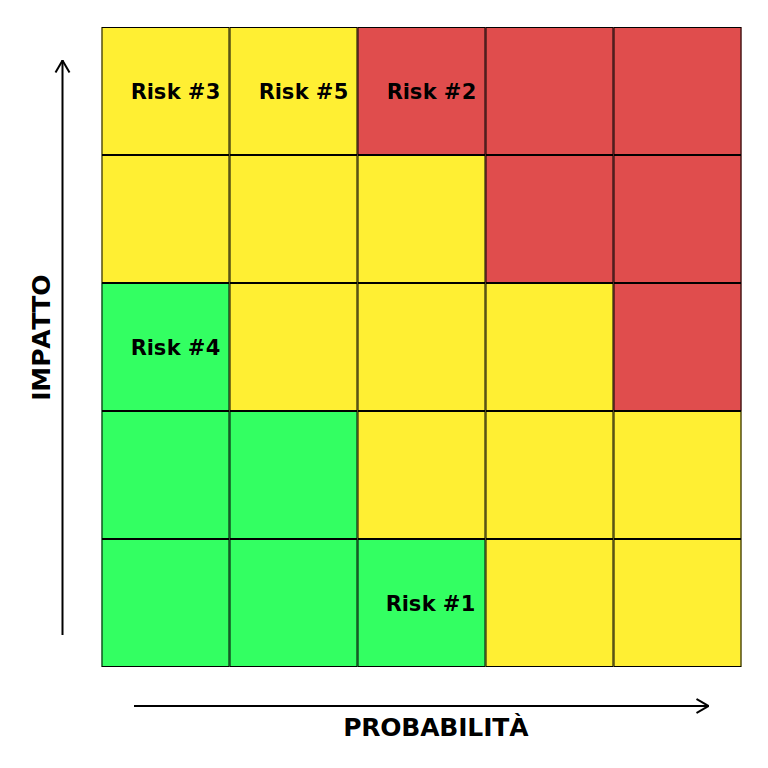
\includegraphics{./Quadrati rischi.svg}
\caption{Quadrati rischi}
\end{figure}

\hypertarget{meccanismo-di-monitoraggio-e-di-controllo}{%
\subsubsection{3.4 Meccanismo di monitoraggio e di
controllo}\label{meccanismo-di-monitoraggio-e-di-controllo}}

Ogni componente del gruppo effetuerà in un primo momento un controllo
personale del lavoro svolto che verrà poi revisionato insieme al resto
del gruppo, dove saranno esposte possibili lacune, imprecisioni e
correzioni possibili.

Ogni settimana si terrà una riunione dove si discute del lavoro svolto
fino a quel punto, se il progetto è in linea con i tempi e sta
proseguendo nella direzione corretta.

Il team di sviluppo ha scelto di appogiarsi a \emph{Github} per lo
sviluppo software e l'organizzazione dei documenti. Per un rapido
scambio di informazioni e comunicazioni urgenti, nel caso occorressero,
verrano utilizzate applicazioni di messagistica come \emph{Telegram}.

\hypertarget{pianificazione-dello-staff}{%
\subsubsection{3.5 Pianificazione dello
staff}\label{pianificazione-dello-staff}}

Lo staff tecnico verrà diviso in due sezioni: una che seguirà lo
sviluppo e l'analisi del robot e una che seguirà l'app Android, questo
per l'elevata differenza di software e capacità necessarie per
sviluppare le due parti.

Lo staff cercherà di lavorare nella maniera più parallela possibile, per
accellerare i tempi. Tutti i lavori fatti dal gruppo saranno depositati
su un repository su Github, dato che ci permetterà di lavorare su
singoli file in parallelo, dove all'occorrenza sarà possibile aprire
Issues e fare commenti sul codice e sulla documentazione depositata.

Nel caso di lacune nelle conoscenze del gruppo verrano colmate
attraverso guide online, tutorial e documentazione ufficiale.

\hypertarget{processi-tecnici}{%
\subsection{4. Processi Tecnici}\label{processi-tecnici}}

\hypertarget{metodi-strumenti-e-tecniche}{%
\subsubsection{4.1 Metodi, strumenti e
tecniche}\label{metodi-strumenti-e-tecniche}}

\begin{itemize}
\tightlist
\item
  \textbf{Strumenti Hardware}:

  \begin{itemize}
  \tightlist
  \item
    Ogni membro del gruppo utilizzerà il proprio notebook personale
    (\emph{Windows}/\emph{Linux}/\emph{Mac}) per lo sviluppo del
    progetto.
  \item
    Ogni membro del gruppo avrà a disposizione il proprio smartphone
    \emph{Android} per lo sviluppo dell'applicazione.
  \item
    \emph{Lego Mindstorms EV3} fornito dall'università.
  \item
    Eventuali sensori aggiuntivi e dongle USB.
  \end{itemize}
\item
  \textbf{Strumenti Software}

  \begin{itemize}
  \tightlist
  \item
    \emph{Git\footnote{\emph{Git}: software di \emph{Code versioning}
      che permette di tenere traccia delle versioni dei file in maniera
      decentralizzata.}}
  \item
    \emph{Android Studio\footnote{\emph{Android studio}: un ambiente di
      sviluppo integrato (IDE) basato sul software di \emph{JetBrains
      IntelliJ IDEA} esclusivamente per la creazione di applicazioni
      \emph{Android{[}\^{}1{]}} native.}}
  \item
    \emph{Typora\footnote{\emph{Typora}: software per la creazione di
      documenti in \emph{Markdown}.}}
  \item
    \emph{CLion\footnote{\emph{CLion}: IDE di Jetbrains dedicato alla
      scrittura di codice C++.}}
  \item
    \emph{Visual Studio Code\footnote{\emph{Visual Studio Code}: IDE
      gratuito di Microsoft.}}
  \item
    \emph{Adobe Xd\footnote{\emph{Adobe Xd}: software gratuito per la
      realizzazione e il mockup delle interfacce grafiche.}}
  \item
    \emph{Docker\footnote{\emph{Docker}: software di virtualizzazione
      che facilita il lavoro di \emph{cross compiling} e
      \emph{deployment}.}}
  \end{itemize}
\end{itemize}

\hypertarget{documentazione-del-software}{%
\subsubsection{4.2 Documentazione del
Software}\label{documentazione-del-software}}

Il progetto sará accompagnato dai seguenti documenti:

\begin{itemize}
\tightlist
\item
  Piano di Progetto
\item
  Documento di Progettazione
\item
  Documento di analisi e specifica
\item
  Piano di Testing
\end{itemize}

\hypertarget{funzionalita-al-supporto-del-progetto}{%
\subsubsection{4.3 Funzionalita al supporto del
progetto}\label{funzionalita-al-supporto-del-progetto}}

\begin{itemize}
\item
  \textbf{Pianificazione della qualitá}

  Lavoreremo in 2 gruppi (uno per il robot e l'altro per l'applicazione)
  che scriveranno e revisioneranno il codice contemporaneamente (in modo
  da minimizzare gli errori) e solo dopo il dovuto testing aggiorneranno
  la documentazione, come previsto dalla metodologia \emph{Agile}.
\item
  \textbf{Pianificazione di Code Version Control e Continuos
  Integration}

  \begin{itemize}
  \item
    Utilizzeremo \emph{Github} in modo da: facilitare il lavoro del
    gruppo in fase di sviluppo / debugging e da tener traccia di tutte
    le versioni precedenti con facilitá.
  \item
    Utilizzeremo strumenti di CI\footnote{\emph{Continuos Integration}:
      software per automatizzare il processo di testing automatico,
      formattazione del codice, validazione e deployment, integrato con
      Git.} in modo da assicurare la qualità del codice ed evitare
    errori di regressione in maniera efficiente.
  \end{itemize}
\end{itemize}

\hypertarget{pianificazione-del-lavoro-delle-risorse-umane-e-del-budget}{%
\subsection{5. Pianificazione del lavoro delle risorse umane e del
budget}\label{pianificazione-del-lavoro-delle-risorse-umane-e-del-budget}}

\hypertarget{wbs}{%
\subsubsection{5.1 WBS}\label{wbs}}

\begin{itemize}
\tightlist
\item
  \textbf{1 PIANIFICAZIONE}

  \begin{itemize}
  \tightlist
  \item
    1.1 Definizione degli obiettivi generali
  \item
    1.2 Definizione del piano di progetto

    \begin{itemize}
    \tightlist
    \item
      1.2.1 Analisi dei processi gestionali
    \item
      1.2.2 Analisi dei processi tecnici
    \item
      1.2.3 Pianificazione del lavoro, delle risorse umane e del budget
    \end{itemize}
  \item
    1.3 Definizione del documento di analisi e specifica
  \end{itemize}
\item
  \textbf{2 PROGETTAZIONE}

  \begin{itemize}
  \tightlist
  \item
    2.1 Definizione del documento di progettazione

    \begin{itemize}
    \tightlist
    \item
      2.1.1 Analisi del sistema
    \item
      2.1.2 Analisi del componente Lego Mindstorms
    \item
      2.1.3 Analisi dell'applicazione Android
    \item
      2.1.4 Prototipazione dell'interfaccia grafica
    \end{itemize}
  \item
    2.2 Definizione del piano di testing
  \end{itemize}
\item
  \textbf{3 REALIZZAZIONE}

  \begin{itemize}
  \tightlist
  \item
    3.1 Apprendimento tecnico
  \item
    3.2 Realizzazione del componente Lego Mindstorms

    \begin{itemize}
    \tightlist
    \item
      3.2.1 Assemblaggio dei componenti hardware
    \item
      3.2.2 Programmazione del firmware
    \end{itemize}
  \item
    3.3 Realizzazione dell'applicazione Android

    \begin{itemize}
    \tightlist
    \item
      3.3.1 Programmazione del backend
    \item
      3.3.2 Programmazione del frontend
    \end{itemize}
  \item
    3.4 Collaudo del sistema
  \end{itemize}
\item
  \textbf{4 DISPIEGAMENTO}

  \begin{itemize}
  \tightlist
  \item
    4.1 Realizzazione del manuale utente
  \item
    4.2 Consegna del sistema
  \end{itemize}
\item
  \textbf{5 REVISIONE}

  \begin{itemize}
  \tightlist
  \item
    5.1 Revisione finale
  \item
    5.2 Chiusura del progetto
  \end{itemize}
\end{itemize}

\hypertarget{dipendenze}{%
\subsubsection{5.2 Dipendenze}\label{dipendenze}}

\begin{longtable}[]{@{}llll@{}}
\toprule
N & Attività & Durata (in ore) & Dipendenze\tabularnewline
\midrule
\endhead
A & Definizione degli obiettivi generali & 5 & -\tabularnewline
B & Analisi dei processi gestionali & 10 & A\tabularnewline
C & Analisi dei processi tecnici & 10 & A\tabularnewline
D & Pianificazione del lavoro, delle risorse umane e del budget & 10 &
A\tabularnewline
E & Definizione del documento di analisi e specifica & 10 & B, C,
D\tabularnewline
F & Analisi del sistema & 10 & E\tabularnewline
G & Analisi del componente Lego Mindstorms & 5 & F\tabularnewline
H & Analisi dell'applicazione Android & 10 & F\tabularnewline
I & Prototipazione dell'interfaccia grafica & 10 & F\tabularnewline
J & Definizione del piano di testing & 10 & G, H, I\tabularnewline
K & Apprendimento tecnico & 15 & J\tabularnewline
L & Assemblaggio dei componenti hardware & 5 & K\tabularnewline
M & Programmazione del firmware & 15 & K\tabularnewline
N & Programmazione del backend & 15 & K\tabularnewline
O & Programmazione del frontend & 10 & K\tabularnewline
P & Collaudo del sistema & 5 & L, M, N, O\tabularnewline
Q & Realizzazione del manuale utente & 10 & P\tabularnewline
R & Consegna del sistema & 1 & Q\tabularnewline
S & Revisione finale & 2 & R\tabularnewline
T & Chiusura del progetto & 1 & S\tabularnewline
\bottomrule
\end{longtable}

\hypertarget{risorse-necessarie}{%
\subsubsection{5.3 Risorse necessarie}\label{risorse-necessarie}}

Le risorse necessarie per la realizzazione del progetto sono: -
\textbf{Risorse umane}: i membri del team di sviluppo e testing e i
responsabili di gestione progetto; - \textbf{Risorse hardware}: un
computer connesso ad Internet per ogni membro del team, hardware
necessario per il robot; - \textbf{Risorse software}: \emph{Telegram}
(comunicazione), \emph{Discord} (comunicazione), \emph{GitHub} (gestione
delle versioni del progetto), \emph{Typora} (stesura della
documentazione), \emph{Latex} (impaginazione della documentazione),
\emph{gcc} (compilazione firmware), \emph{CMake} (automazione della
compilazione), \emph{VSCode} (programmazione del firmware),
\emph{Android Studio} (programmazione dell'applicazione Android).

\hypertarget{allocazione-del-budget-e-delle-risorse}{%
\subsubsection{5.4 Allocazione del budget e delle
risorse}\label{allocazione-del-budget-e-delle-risorse}}

Lo sviluppo dell'applicazione non richiede alcun tipo di risorsa
economica, in quanto i software impiegati per la realizzazione sono a
costo zero. Inoltre, anche il set Lego Mindstorms EV3 è stato fornito in
comodato d'uso dall'Università Ca' Foscari.

Eventuali sensori esterni saranno acquistati dai componenti del progetto
in maniera volontaria e indipendente e non saranno considerati nel
budget di progetto.

\hypertarget{pianificazione}{%
\subsubsection{5.5 Pianificazione}\label{pianificazione}}

La pianificazione del progetto è basata sui termini di consegna del
progetto e di tutta la relativa documentazione, stabiliti con il
professor Cortesi all'interno del corso di Ingegneria del Software
2018/2019: - Piano di Progetto: 16/10/2018 - Documento di Analisi e
Specifica: 02/11/2018 - ­Piano di Testing: 15/11/2018 - Documento di
Progettazione: 10/12/2018 - Realizzazione e messa in linea: 31/01/2019

\end{document}
